\section{ACOSH Inverse Hyperbolic Cosine Function}

\subsection{Usage}

Computes the inverse hyperbolic cosine of its argument.  The general
syntax for its use is
\begin{verbatim}
  y = acosh(x)
\end{verbatim}
where \verb|x| is an \verb|n|-dimensional array of numerical type.
\subsection{Function Internals}

The \verb|acosh| function is computed from the formula
\[
   \cosh^{-1}(x) = \log\left(x + (x^2 - 1)^0.5\right)
\]
where the \verb|log| (and square root) is taken in its most general sense.
\subsection{Examples}

Here is a simple plot of the inverse hyperbolic cosine function
\begin{verbatim}
--> x = linspace(1,pi);
--> plot(x,acosh(x)); grid('on');
\end{verbatim}


\centerline{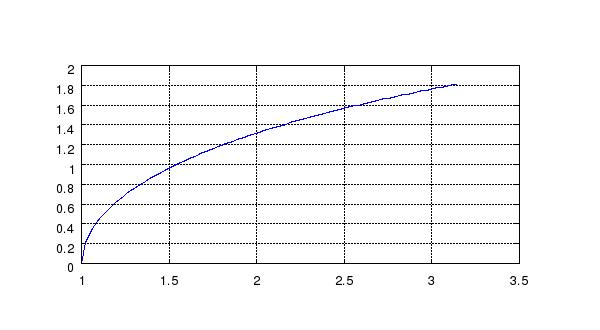
\includegraphics[width=8cm]{acoshplot}}

